\documentclass{article}
\usepackage[utf8]{inputenc}
\usepackage{amsmath}
\usepackage{listings}
\usepackage{geometry}
\usepackage{xcolor}
\usepackage{tikz}
\usepackage{tcolorbox}
\usepackage{amsmath} % For mathematical typesetting

\geometry{margin=1in}

\title{Quplexity: A faster modern quantum computing library \\ written in Assembly.}
\author{Jacob Liam Gill}
\date{July 2024}

\begin{document}

\maketitle

\section*{1. Abstract \& Overview}
Quantum Computer Simulators (QCS's) are often complex pieces of technology where performace is essential.
Most modern QCS's like Qrack and Qiskit are written in either Python or C/C++.
C++ being the more popular and suitable option for performant simulators. Despite C++ being performant and fast in nature, 
x86 and ARM/AMR64 Assembly, when written and utilised correctly proves to be significantly faster than C++ whilst also being extremely lightweight in nature.
This paper looks at how I have successfully utilised the Assembly language to provide performance and "weight" benefits to QCS's and the like. All the code for this project can be viewed on the Quplexity github.

\section*{2. Matrix Math}
In the field of Quantum Computing (QC) mathematical methods involving the manipulation and computation of matrices are very prominent in QCS's.
With this in mind I set out to optimaize matrix math in Assembly for Intel and ARM/ARM64 processors. 

\subsubsection*{2.1 Standard Multiplication of 2x2 Matrices}
This section will explore the benefits of a standard matrices multiplication function written in Assembly opposed to the traditional C++.
The Math that the Assembly function performed can be seen below: \\

\begin{center}
  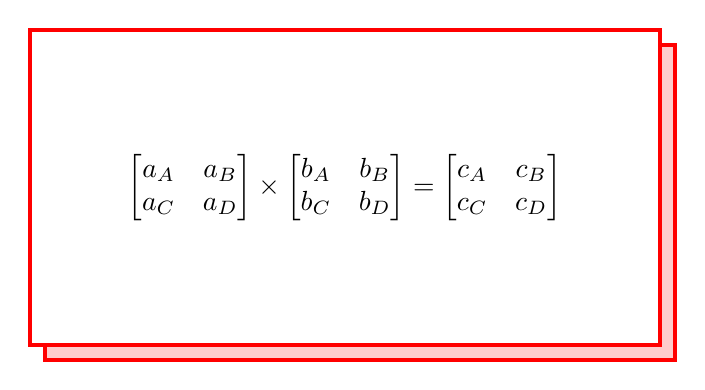
\begin{tikzpicture}
      % Shadow box
      \node[fill=red!20, draw=red, line width=0.5mm, minimum width=8cm, minimum height=4cm, xshift=2mm, yshift=-2mm] at (0,0) {};
  
      % Main box
      \node[fill=white, draw=red, line width=0.5mm, minimum width=8cm, minimum height=4cm] at (0,0) {
          $\begin{bmatrix}
                a_{A} & a_{B} \\
                a_{C} & a_{D}
              \end{bmatrix}
              \times
              \begin{bmatrix}
                b_{A} & b_{B} \\
                b_{C} & b_{D}
              \end{bmatrix}
              = 
              \begin{bmatrix}
                  c_{A} & c_{B} \\
                  c_{C} & c_{D}
              \end{bmatrix}$
      };
  \end{tikzpicture}
\end{center}

\noindent I wrote a C++ function that mirrored my Assembly function, I compared the execution times for both using the C++ "chrono" library.
You can view this function in ./Intel/math.s of the Quplexity github repository, the function is named "\_gills\_matrix2x2".
Below are the calculation and execution time results for Intel: \\

\noindent \fbox{%
  \parbox{\dimexpr\textwidth-2\fboxsep}{%
    \textbf C++ Result: 19 22 43 50 \\
            Assembly Result: 19 22 43 50 \\
            C++ Duration: 0.531 ms \\
            Assembly Duration: 0.108 ms \\
  }%
} \\

\subsubsection*{2.2 Inverse of a 2x2 Matrix}
This is an example of how to use the Quplexity function "gills\_inv\_matrix2x2". It involves finding the determinant of the matrix $\frac{1}{det(A)}$ if $det(a) \neq 0$ then there is a inverse of that matrix.
After the determinant has been calculated the function the multiplys the numbers inside the matrix by $\frac{1}{det(A)}$ to produce the \\
resultant matrix. The mathematics behind this function can be viewed below: \\

\begin{center}
  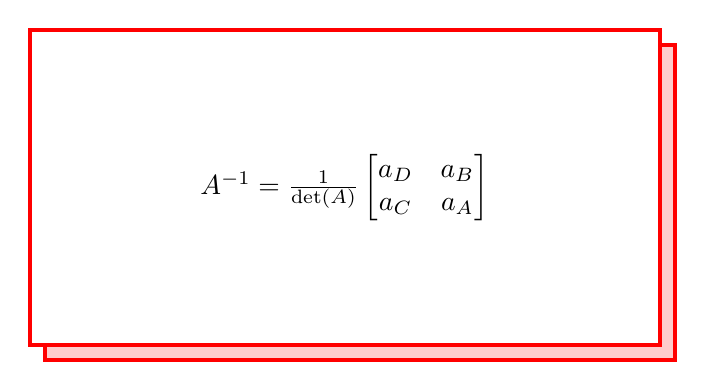
\begin{tikzpicture}
      % Shadow box
      \node[fill=red!20, draw=red, line width=0.5mm, minimum width=8cm, minimum height=4cm, xshift=2mm, yshift=-2mm] at (0,0) {};
  
      % Main box
      \node[fill=white, draw=red, line width=0.5mm, minimum width=8cm, minimum height=4cm] at (0,0) {
          $
            A^{-1} = \frac{1}{\det(A)} \begin{bmatrix}
            a_{D} & a_{B} \\
            a_{C} & a_{A}
            \end{bmatrix}
          $
      };
  \end{tikzpicture}
\end{center}

\end{document}